
%% bare_conf.tex
%% V1.3
%% 2007/01/11
%% by Michael Shell
%% See:
%% http://www.michaelshell.org/
%% for current contact information.
%%
%% This is a skeleton file demonstrating the use of IEEEtran.cls
%% (requires IEEEtran.cls version 1.7 or later) with an IEEE conference paper.
%%
%% Support sites:
%% http://www.michaelshell.org/tex/ieeetran/
%% http://www.ctan.org/tex-archive/macros/latex/contrib/IEEEtran/
%% and
%% http://www.ieee.org/

%%*************************************************************************
%% Legal Notice:
%% This code is offered as-is without any warranty either expressed or
%% implied; without even the implied warranty of MERCHANTABILITY or
%% FITNESS FOR A PARTICULAR PURPOSE! 
%% User assumes all risk.
%% In no event shall IEEE or any contributor to this code be liable for
%% any damages or losses, including, but not limited to, incidental,
%% consequential, or any other damages, resulting from the use or misuse
%% of any information contained here.
%%
%% All comments are the opinions of their respective authors and are not
%% necessarily endorsed by the IEEE.
%%
%% This work is distributed under the LaTeX Project Public License (LPPL)
%% ( http://www.latex-project.org/ ) version 1.3, and may be freely used,
%% distributed and modified. A copy of the LPPL, version 1.3, is included
%% in the base LaTeX documentation of all distributions of LaTeX released
%% 2003/12/01 or later.
%% Retain all contribution notices and credits.
%% ** Modified files should be clearly indicated as such, including  **
%% ** renaming them and changing author support contact information. **
%%
%% File list of work: IEEEtran.cls, IEEEtran_HOWTO.pdf, bare_adv.tex,
%%                    bare_conf.tex, bare_jrnl.tex, bare_jrnl_compsoc.tex
%%*************************************************************************

% *** Authors should verify (and, if needed, correct) their LaTeX system  ***
% *** with the testflow diagnostic prior to trusting their LaTeX platform ***
% *** with production work. IEEE's font choices can trigger bugs that do  ***
% *** not appear when using other class files.                            ***
% The testflow support page is at:
% http://www.michaelshell.org/tex/testflow/



% Note that the a4paper option is mainly intended so that authors in
% countries using A4 can easily print to A4 and see how their papers will
% look in print - the typesetting of the document will not typically be
% affected with changes in paper size (but the bottom and side margins will).
% Use the testflow package mentioned above to verify correct handling of
% both paper sizes by the user's LaTeX system.
%
% Also note that the "draftcls" or "draftclsnofoot", not "draft", option
% should be used if it is desired that the figures are to be displayed in
% draft mode.
%
\documentclass[conference]{IEEEtran}
% Add the compsoc option for Computer Society conferences.
%
% If IEEEtran.cls has not been installed into the LaTeX system files,
% manually specify the path to it like:
% \documentclass[conference]{../sty/IEEEtran}





% Some very useful LaTeX packages include:
% (uncomment the ones you want to load)


% *** MISC UTILITY PACKAGES ***
%
\usepackage{ifpdf}
% Heiko Oberdiek's ifpdf.sty is very useful if you need conditional
% compilation based on whether the output is pdf or dvi.
% usage:
% \ifpdf
%   % pdf code
% \else
%   % dvi code
% \fi
% The latest version of ifpdf.sty can be obtained from:
% http://www.ctan.org/tex-archive/macros/latex/contrib/oberdiek/
% Also, note that IEEEtran.cls V1.7 and later provides a builtin
% \ifCLASSINFOpdf conditional that works the same way.
% When switching from latex to pdflatex and vice-versa, the compiler may
% have to be run twice to clear warning/error messages.






% *** CITATION PACKAGES ***
%
\usepackage{cite}
% cite.sty was written by Donald Arseneau
% V1.6 and later of IEEEtran pre-defines the format of the cite.sty package
% \cite{} output to follow that of IEEE. Loading the cite package will
% result in citation numbers being automatically sorted and properly
% "compressed/ranged". e.g., [1], [9], [2], [7], [5], [6] without using
% cite.sty will become [1], [2], [5]--[7], [9] using cite.sty. cite.sty's
% \cite will automatically add leading space, if needed. Use cite.sty's
% noadjust option (cite.sty V3.8 and later) if you want to turn this off.
% cite.sty is already installed on most LaTeX systems. Be sure and use
% version 4.0 (2003-05-27) and later if using hyperref.sty. cite.sty does
% not currently provide for hyperlinked citations.
% The latest version can be obtained at:
% http://www.ctan.org/tex-archive/macros/latex/contrib/cite/
% The documentation is contained in the cite.sty file itself.






% *** GRAPHICS RELATED PACKAGES ***
%
%\ifCLASSINFOpdf
\usepackage{graphicx}
  % declare the path(s) where your graphic files are
  % \graphicspath{{../pdf/}{../jpeg/}}
  % and their extensions so you won't have to specify these with
  % every instance of \includegraphics
%\DeclareGraphicsExtensions{.pdf,.jpeg,.png}
%\else
  % or other class option (dvipsone, dvipdf, if not using dvips). graphicx
  % will default to the driver specified in the system graphics.cfg if no
  % driver is specified.
  % \usepackage[dvips]{graphicx}
  % declare the path(s) where your graphic files are
  % \graphicspath{{../eps/}}
  % and their extensions so you won't have to specify these with
  % every instance of \includegraphics
  % \DeclareGraphicsExtensions{.eps}
%\fi
% graphicx was written by David Carlisle and Sebastian Rahtz. It is
% required if you want graphics, photos, etc. graphicx.sty is already
% installed on most LaTeX systems. The latest version and documentation can
% be obtained at: 
% http://www.ctan.org/tex-archive/macros/latex/required/graphics/
% Another good source of documentation is "Using Imported Graphics in
% LaTeX2e" by Keith Reckdahl which can be found as epslatex.ps or
% epslatex.pdf at: http://www.ctan.org/tex-archive/info/
%
% latex, and pdflatex in dvi mode, support graphics in encapsulated
% postscript (.eps) format. pdflatex in pdf mode supports graphics
% in .pdf, .jpeg, .png and .mps (metapost) formats. Users should ensure
% that all non-photo figures use a vector format (.eps, .pdf, .mps) and
% not a bitmapped formats (.jpeg, .png). IEEE frowns on bitmapped formats
% which can result in "jaggedy"/blurry rendering of lines and letters as
% well as large increases in file sizes.
%
% You can find documentation about the pdfTeX application at:
% http://www.tug.org/applications/pdftex





% *** MATH PACKAGES ***
%
%\usepackage[cmex10]{amsmath}
% A popular package from the American Mathematical Society that provides
% many useful and powerful commands for dealing with mathematics. If using
% it, be sure to load this package with the cmex10 option to ensure that
% only type 1 fonts will utilized at all point sizes. Without this option,
% it is possible that some math symbols, particularly those within
% footnotes, will be rendered in bitmap form which will result in a
% document that can not be IEEE Xplore compliant!
%
% Also, note that the amsmath package sets \interdisplaylinepenalty to 10000
% thus preventing page breaks from occurring within multiline equations. Use:
%\interdisplaylinepenalty=2500
% after loading amsmath to restore such page breaks as IEEEtran.cls normally
% does. amsmath.sty is already installed on most LaTeX systems. The latest
% version and documentation can be obtained at:
% http://www.ctan.org/tex-archive/macros/latex/required/amslatex/math/





% *** SPECIALIZED LIST PACKAGES ***
%
%\usepackage{algorithmic}
% algorithmic.sty was written by Peter Williams and Rogerio Brito.
% This package provides an algorithmic environment fo describing algorithms.
% You can use the algorithmic environment in-text or within a figure
% environment to provide for a floating algorithm. Do NOT use the algorithm
% floating environment provided by algorithm.sty (by the same authors) or
% algorithm2e.sty (by Christophe Fiorio) as IEEE does not use dedicated
% algorithm float types and packages that provide these will not provide
% correct IEEE style captions. The latest version and documentation of
% algorithmic.sty can be obtained at:
% http://www.ctan.org/tex-archive/macros/latex/contrib/algorithms/
% There is also a support site at:
% http://algorithms.berlios.de/index.html
% Also of interest may be the (relatively newer and more customizable)
% algorithmicx.sty package by Szasz Janos:
% http://www.ctan.org/tex-archive/macros/latex/contrib/algorithmicx/




% *** ALIGNMENT PACKAGES ***
%
%\usepackage{array}
% Frank Mittelbach's and David Carlisle's array.sty patches and improves
% the standard LaTeX2e array and tabular environments to provide better
% appearance and additional user controls. As the default LaTeX2e table
% generation code is lacking to the point of almost being broken with
% respect to the quality of the end results, all users are strongly
% advised to use an enhanced (at the very least that provided by array.sty)
% set of table tools. array.sty is already installed on most systems. The
% latest version and documentation can be obtained at:
% http://www.ctan.org/tex-archive/macros/latex/required/tools/


%\usepackage{mdwmath}
%\usepackage{mdwtab}
% Also highly recommended is Mark Wooding's extremely powerful MDW tools,
% especially mdwmath.sty and mdwtab.sty which are used to format equations
% and tables, respectively. The MDWtools set is already installed on most
% LaTeX systems. The lastest version and documentation is available at:
% http://www.ctan.org/tex-archive/macros/latex/contrib/mdwtools/


% IEEEtran contains the IEEEeqnarray family of commands that can be used to
% generate multiline equations as well as matrices, tables, etc., of high
% quality.


%\usepackage{eqparbox}
% Also of notable interest is Scott Pakin's eqparbox package for creating
% (automatically sized) equal width boxes - aka "natural width parboxes".
% Available at:
% http://www.ctan.org/tex-archive/macros/latex/contrib/eqparbox/





% *** SUBFIGURE PACKAGES ***
%\usepackage[tight,footnotesize]{subfigure}
% subfigure.sty was written by Steven Douglas Cochran. This package makes it
% easy to put subfigures in your figures. e.g., "Figure 1a and 1b". For IEEE
% work, it is a good idea to load it with the tight package option to reduce
% the amount of white space around the subfigures. subfigure.sty is already
% installed on most LaTeX systems. The latest version and documentation can
% be obtained at:
% http://www.ctan.org/tex-archive/obsolete/macros/latex/contrib/subfigure/
% subfigure.sty has been superceeded by subfig.sty.



%\usepackage[caption=false]{caption}
%\usepackage[font=footnotesize]{subfig}
% subfig.sty, also written by Steven Douglas Cochran, is the modern
% replacement for subfigure.sty. However, subfig.sty requires and
% automatically loads Axel Sommerfeldt's caption.sty which will override
% IEEEtran.cls handling of captions and this will result in nonIEEE style
% figure/table captions. To prevent this problem, be sure and preload
% caption.sty with its "caption=false" package option. This is will preserve
% IEEEtran.cls handing of captions. Version 1.3 (2005/06/28) and later 
% (recommended due to many improvements over 1.2) of subfig.sty supports
% the caption=false option directly:
%\usepackage[caption=false,font=footnotesize]{subfig}
%
% The latest version and documentation can be obtained at:
% http://www.ctan.org/tex-archive/macros/latex/contrib/subfig/
% The latest version and documentation of caption.sty can be obtained at:
% http://www.ctan.org/tex-archive/macros/latex/contrib/caption/




% *** FLOAT PACKAGES ***
%
%\usepackage{fixltx2e}
% fixltx2e, the successor to the earlier fix2col.sty, was written by
% Frank Mittelbach and David Carlisle. This package corrects a few problems
% in the LaTeX2e kernel, the most notable of which is that in current
% LaTeX2e releases, the ordering of single and double column floats is not
% guaranteed to be preserved. Thus, an unpatched LaTeX2e can allow a
% single column figure to be placed prior to an earlier double column
% figure. The latest version and documentation can be found at:
% http://www.ctan.org/tex-archive/macros/latex/base/



%\usepackage{stfloats}
% stfloats.sty was written by Sigitas Tolusis. This package gives LaTeX2e
% the ability to do double column floats at the bottom of the page as well
% as the top. (e.g., "\begin{figure*}[!b]" is not normally possible in
% LaTeX2e). It also provides a command:
%\fnbelowfloat
% to enable the placement of footnotes below bottom floats (the standard
% LaTeX2e kernel puts them above bottom floats). This is an invasive package
% which rewrites many portions of the LaTeX2e float routines. It may not work
% with other packages that modify the LaTeX2e float routines. The latest
% version and documentation can be obtained at:
% http://www.ctan.org/tex-archive/macros/latex/contrib/sttools/
% Documentation is contained in the stfloats.sty comments as well as in the
% presfull.pdf file. Do not use the stfloats baselinefloat ability as IEEE
% does not allow \baselineskip to stretch. Authors submitting work to the
% IEEE should note that IEEE rarely uses double column equations and
% that authors should try to avoid such use. Do not be tempted to use the
% cuted.sty or midfloat.sty packages (also by Sigitas Tolusis) as IEEE does
% not format its papers in such ways.





% *** PDF, URL AND HYPERLINK PACKAGES ***
%
%\usepackage{url}
% url.sty was written by Donald Arseneau. It provides better support for
% handling and breaking URLs. url.sty is already installed on most LaTeX
% systems. The latest version can be obtained at:
% http://www.ctan.org/tex-archive/macros/latex/contrib/misc/
% Read the url.sty source comments for usage information. Basically,
% \url{my_url_here}.


\usepackage{pbox}


% *** Do not adjust lengths that control margins, column widths, etc. ***
% *** Do not use packages that alter fonts (such as pslatex).         ***
% There should be no need to do such things with IEEEtran.cls V1.6 and later.
% (Unless specifically asked to do so by the journal or conference you plan
% to submit to, of course. )

% *** SOURCE CODE LISTINGS ***
\usepackage{listings}
\usepackage{ifthen}
\usepackage{libertine} % for the pretty dark-circle-enclosed numbers
\usepackage{fontspec}
\usepackage{fancybox}
\newfontfamily{\lstsansserif}[Scale=.7]{Arial}
\newfontfamily{\textlst}{Arial}
\newcounter{lstNoteCounter}
\newcommand{\lnnum}[1]
    {\ifthenelse{#1 =  1}{\libertineGlyph{uni2776}}
    {\ifthenelse{#1 =  2}{\libertineGlyph{uni2777}}
    {\ifthenelse{#1 =  3}{\libertineGlyph{uni2778}}
    {\ifthenelse{#1 =  4}{\libertineGlyph{uni2779}}
    {\ifthenelse{#1 =  5}{\libertineGlyph{uni277A}}
    {\ifthenelse{#1 =  6}{\libertineGlyph{uni277B}}
    {\ifthenelse{#1 =  7}{\libertineGlyph{uni277C}}
    {\ifthenelse{#1 =  8}{\libertineGlyph{uni277D}}
    {\ifthenelse{#1 =  9}{\libertineGlyph{uni277E}}
    {\ifthenelse{#1 = 10}{\libertineGlyph{uni277F}}
    {\ifthenelse{#1 = 11}{\libertineGlyph{uni24EB}}
    {\ifthenelse{#1 = 12}{\libertineGlyph{uni24EC}}
    {\ifthenelse{#1 = 13}{\libertineGlyph{uni24ED}}
    {\ifthenelse{#1 = 14}{\libertineGlyph{uni24EE}}
    {\ifthenelse{#1 = 15}{\libertineGlyph{uni24EF}}
    {\ifthenelse{#1 = 16}{\libertineGlyph{uni24F0}}
    {\ifthenelse{#1 = 17}{\libertineGlyph{uni24F1}}
    {\ifthenelse{#1 = 18}{\libertineGlyph{uni24F2}}
    {\ifthenelse{#1 = 19}{\libertineGlyph{uni24F3}}
    {\ifthenelse{#1 = 20}{\libertineGlyph{uni24F4}}
    {?}}}}}}}}}}}}}}}}}}}}}


\newcommand{\lstref}[1]{\lnnum{\ref{#1}}}

\newcommand{\lstnote}[1] {
\label{#1}\vbox{\llap{{\lnnum{\ref{#1}}}\hskip 1em}}
}

\lstnewenvironment{csource}[1][]
{
 \setcounter{lstNoteCounter}{0}
 \lstset{basicstyle=\lstsansserif, frame=lines, framexleftmargin=0.5em,
            framexrightmargin=0.5em, showstringspaces=false, escapeinside={(*@}{@*)}, #1}
}{}


% correct bad hyphenation here
\hyphenation{op-tical net-works semi-conduc-tor}


\begin{document}
%
% paper title
% can use linebreaks \\ within to get better formatting as desired
\title{Bare Demo of IEEEtran.cls for Conferences}


% author names and affiliations
% use a multiple column layout for up to three different
% affiliations
\author{\IEEEauthorblockN{Michael Shell}
\IEEEauthorblockA{School of Electrical and\\Computer Engineering\\
Georgia Institute of Technology\\
Atlanta, Georgia 30332--0250\\
Email: http://www.michaelshell.org/contact.html}
\and
\IEEEauthorblockN{Homer Simpson}
\IEEEauthorblockA{Twentieth Century Fox\\
Springfield, USA\\
Email: homer@thesimpsons.com}
\and
\IEEEauthorblockN{James Kirk\\ and Montgomery Scott}
\IEEEauthorblockA{Starfleet Academy\\
San Francisco, California 96678-2391\\
Telephone: (800) 555--1212\\
Fax: (888) 555--1212}}

% conference papers do not typically use \thanks and this command
% is locked out in conference mode. If really needed, such as for
% the acknowledgment of grants, issue a \IEEEoverridecommandlockouts
% after \documentclass

% for over three affiliations, or if they all won't fit within the width
% of the page, use this alternative format:
% 
%\author{\IEEEauthorblockN{Michael Shell\IEEEauthorrefmark{1},
%Homer Simpson\IEEEauthorrefmark{2},
%James Kirk\IEEEauthorrefmark{3}, 
%Montgomery Scott\IEEEauthorrefmark{3} and
%Eldon Tyrell\IEEEauthorrefmark{4}}
%\IEEEauthorblockA{\IEEEauthorrefmark{1}School of Electrical and Computer Engineering\\
%Georgia Institute of Technology,
%Atlanta, Georgia 30332--0250\\ Email: see http://www.michaelshell.org/contact.html}
%\IEEEauthorblockA{\IEEEauthorrefmark{2}Twentieth Century Fox, Springfield, USA\\
%Email: homer@thesimpsons.com}
%\IEEEauthorblockA{\IEEEauthorrefmark{3}Starfleet Academy, San Francisco, California 96678-2391\\
%Telephone: (800) 555--1212, Fax: (888) 555--1212}
%\IEEEauthorblockA{\IEEEauthorrefmark{4}Tyrell Inc., 123 Replicant Street, Los Angeles, California 90210--4321}}




% use for special paper notices
%\IEEEspecialpapernotice{(Invited Paper)}




% make the title area
\maketitle

\begin{abstract}
  We present a context-oriented approach to develop self-adaptive
  software for extremely resource-constrained cyber-physical systems
  (CPSs). % These are sensing and actuating systems deployed in the
  % physical world whose operation is controlled by a computing and
  % communication core.
  Because of unpredictable environment dynamics, CPS software must be
  designed and implemented to dynamically adapt to widely different
  situations. Our approach provides design concepts and language
  support to achieve this against extreme resource constraints. To
  this end, we bring a notion of context-oriented design and
  programming down to platforms with only a few KBytes of memory and
  currently leveraging rather basic programming environments. Early
  results demonstrate that our approach greatly simplifies the design
  and implementation of adaptive CPS software at the price of a modest
  system overhead. To our knowledge, we are the first to enable
  context-oriented design and programming in similarly-constrained
  platforms.
\end{abstract}


%%% Local Variables: 
%%% mode: latex
%%% TeX-master: "paper"
%%% End: 


% IEEEtran.cls defaults to using nonbold math in the Abstract.
% This preserves the distinction between vectors and scalars. However,
% if the conference you are submitting to favors bold math in the abstract,
% then you can use LaTeX's standard command \boldmath at the very start
% of the abstract to achieve this. Many IEEE journals/conferences frown on
% math in the abstract anyway.

% no keywords




% For peer review papers, you can put extra information on the cover
% page as needed:
% \ifCLASSOPTIONpeerreview
% \begin{center} \bfseries EDICS Category: 3-BBND \end{center}
% \fi
%
% For peerreview papers, this IEEEtran command inserts a page break and
% creates the second title. It will be ignored for other modes.
\IEEEpeerreviewmaketitle

\section{Introduction}
% no \IEEEPARstart
This demo file is intended to serve as a ``starter file''
for IEEE conference papers produced under \LaTeX\ using
IEEEtran.cls version 1.7 and later.
% You must have at least 2 lines in the paragraph with the drop letter
% (should never be an issue)
I wish you the best of success.

\hfill mds
 
\hfill January 11, 2007

\subsection{Subsection Heading Here}
Subsection text here.


\subsubsection{Subsubsection Heading Here}
Subsubsection text here.


% An example of a floating figure using the graphicx package.
% Note that \label must occur AFTER (or within) \caption.
% For figures, \caption should occur after the \includegraphics.
% Note that IEEEtran v1.7 and later has special internal code that
% is designed to preserve the operation of \label within \caption
% even when the captionsoff option is in effect. However, because
% of issues like this, it may be the safest practice to put all your
% \label just after \caption rather than within \caption{}.
%
% Reminder: the "draftcls" or "draftclsnofoot", not "draft", class
% option should be used if it is desired that the figures are to be
% displayed while in draft mode.
%
%\begin{figure}[!t]
%\centering
%\includegraphics[width=2.5in]{myfigure}
% where an .eps filename suffix will be assumed under latex, 
% and a .pdf suffix will be assumed for pdflatex; or what has been declared
% via \DeclareGraphicsExtensions.
%\caption{Simulation Results}
%\label{fig_sim}
%\end{figure}

% Note that IEEE typically puts floats only at the top, even when this
% results in a large percentage of a column being occupied by floats.


% An example of a double column floating figure using two subfigures.
% (The subfig.sty package must be loaded for this to work.)
% The subfigure \label commands are set within each subfloat command, the
% \label for the overall figure must come after \caption.
% \hfil must be used as a separator to get equal spacing.
% The subfigure.sty package works much the same way, except \subfigure is
% used instead of \subfloat.
%
%\begin{figure*}[!t]
%\centerline{\subfloat[Case I]\includegraphics[width=2.5in]{subfigcase1}%
%\label{fig_first_case}}
%\hfil
%\subfloat[Case II]{\includegraphics[width=2.5in]{subfigcase2}%
%\label{fig_second_case}}}
%\caption{Simulation results}
%\label{fig_sim}
%\end{figure*}
%
% Note that often IEEE papers with subfigures do not employ subfigure
% captions (using the optional argument to \subfloat), but instead will
% reference/describe all of them (a), (b), etc., within the main caption.


% An example of a floating table. Note that, for IEEE style tables, the 
% \caption command should come BEFORE the table. Table text will default to
% \footnotesize as IEEE normally uses this smaller font for tables.
% The \label must come after \caption as always.
%
%\begin{table}[!t]
%% increase table row spacing, adjust to taste
%\renewcommand{\arraystretch}{1.3}
% if using array.sty, it might be a good idea to tweak the value of
% \extrarowheight as needed to properly center the text within the cells
%\caption{An Example of a Table}
%\label{table_example}
%\centering
%% Some packages, such as MDW tools, offer better commands for making tables
%% than the plain LaTeX2e tabular which is used here.
%\begin{tabular}{|c||c|}
%\hline
%One & Two\\
%\hline
%Three & Four\\
%\hline
%\end{tabular}
%\end{table}


% Note that IEEE does not put floats in the very first column - or typically
% anywhere on the first page for that matter. Also, in-text middle ("here")
% positioning is not used. Most IEEE journals/conferences use top floats
% exclusively. Note that, LaTeX2e, unlike IEEE journals/conferences, places
% footnotes above bottom floats. This can be corrected via the \fnbelowfloat
% command of the stfloats package.
\section{Context Oriented Programming}\label{sec:cop}
To mention: definition of Context, definition of COP, main ingredients of COP.

Recently introduced Context-oriented programming (COP)~\cite{Hirschfeld08} has
proven its effectiveness in creating context-aware software, such as graphical
user interface~\cite{Keays03}, text editor~\cite{Kamina11}, and even software for wireless
sensor networks~\cite{Sehic11}, in high-level though. COP paradigm has been
implemented in different languages~\cite{Salvaneschi12} by modifying them both
syntactically and semantically. Practically, COP brings a language-level abstraction 
to enable the expression of behavioral variation in the host language.

To provide context-oriented adaptation, language should satisfy certain requirements, such as
possibility to define behavioral variations, group and activate them at
run-time. Despite there are different methods to satisfy these
requirements~\cite{Salvaneschi12}, the main ingredients are \emph{context} and
\emph{layered functions}. The latter -- the implementations of behavioral
variations -- depend on the \emph{context} -- the information which is
computationally accessible.

We adopt notions and adaptation techniques used in existing COP implementations,
and bring them down to low-level programming for WSNs. Our language \conesc --
which is discussed in the next section in details -- is based on nesC and extend
it by adding context-oriented notions. Basically, we extend the syntax to
specify the behavioral variation of the software, group them into modules and
activate them at run-time.

\newsavebox{\boxcc}
\Savebox{\boxcc}{
\hspace{-0.25cm}
\begin{minipage}[l]{\columnwidth}
\begin{lstlisting}[style=conescframe]
context group BaseStationG {
*\lstnote{layereddef}* layered command void report(msg_t msg);
}implementation {
*\lstnote{contexts}* contexts Reachable,
*\lstnote{isdefault}*          Unreachable is default,
*\lstnote{iserror}*          MyErrorC is error;
 components Routing, Logging;
 Reachable.Collection -> Routing;
 Unreachable.DataStore -> Logging;}
\end{lstlisting}
\end{minipage}
}
\newsavebox{\boxbscm}
\Savebox{\boxbscm}{
\hspace{-0.25cm}
\begin{minipage}[l]{\columnwidth}
\begin{lstlisting}[style=conescframe]
module BaseStationContextManager {
 uses context group BaseStationG;
}implementation {
 event msg_t Beacon.receive(msg_t msg) {
*\lstnote{actBS}*  activate BaseStationG.Reachable;
  call BSReset.stop(); 
  call BSReset.startOneShot(TIMEOUT);}
 event void BSReset.fired() {
*\lstnote{actNoBS}*  activate BaseStationG.Unreachable;}}
\end{lstlisting}
\end{minipage}
}
\newsavebox{\boxc}
\Savebox{\boxc}{
\hspace{-0.25cm}
\begin{minipage}[l]{\columnwidth}
\begin{lstlisting}[style=conescframe]
context Unreachable {
*\lstnote{dependence}* transitions Reachable iff ActivityG.Running;
 uses interface DataStore;
}implementation {
*\lstnote{activatedUnreachable}* event void activated(){//...}
*\lstnote{deactivatedUnreachable}* event void deactivated(){//...}
*\lstnote{checkUnreachable}* command bool check(){//...}
 layered command void report(msg_t msg){
*\lstnote{layeredimp}*  call DataStore.deposit(msg);}}
\end{lstlisting}
\end{minipage}
}
\newsavebox{\boxirc}
\Savebox{\boxirc}{
\hspace{-0.25cm}
\begin{minipage}[l]{\columnwidth}
\begin{lstlisting}[style=conescframe]
context Reachable {
 uses interface Collection;
 uses context group BatteryG; 
}implementation {
*\lstnote{activated}* event void activated(){ 
  call GPS.stop();}
*\lstnote{deactivated}* event void deactivated(){//...}
*\lstnote{check}* command bool check(){
  return call BatteryG.getContext() == BatteryG.Normal;}
 layered command void report(msg_t msg){
*\lstnote{layeredimp2}*  call Collection.send(msg);}}
\end{lstlisting}
\end{minipage}
}
\newsavebox{\boxlc}
\Savebox{\boxlc}{
\hspace{-0.25cm}
\begin{minipage}[l]{\columnwidth}
\begin{lstlisting}[style=conescframe]
context Low {
*\lstnote{triggers}* triggers BaseStationG.Unreachable;
}implementation {//...}
\end{lstlisting}
\end{minipage}
}
% \newsavebox{\boxmc}
% \Savebox{\boxmc}{
% \hspace{-0.25cm}
% \begin{minipage}[l]{\columnwidth}
% \begin{lstlisting}[style=conescframe]
% configuration ApplicationC {
% }implementation {
% *\lstnote{declaration}* components BaseStationG, Application;
%  //...
% *\lstnote{wiring}* Application.BaseStationG -> BaseStationG;}
% \end{lstlisting}
% \end{minipage}
% }
\newsavebox{\boxmm}
\Savebox{\boxmm}{
\hspace{-0.25cm}
\begin{minipage}[l]{\columnwidth}
\begin{lstlisting}[style=conescframe]
module User {
*\lstnote{cgdecl}* uses context group BaseStationG;
}implementation {
 event void Timer.fired() {
*\lstnote{calling}*  call BaseStationG.report(msg);}
*\lstnote{eventCC}* event void BaseStationG.contextChanged(context_t con) {
*\lstnote{concheck}*  if(con == BaseStationG.Reachable) // DO SOMETHING...}}
\end{lstlisting}
\end{minipage}
}
\newsavebox{\boxnmc}
\Savebox{\boxnmc}{
\hspace{-0.25cm}
\begin{minipage}[l]{\columnwidth}
\begin{lstlisting}[style=conescframe]
context NotMoving {
*\lstnote{transitions}* transitions Resting;
}implementation {//...}
\end{lstlisting}
\end{minipage}
}
\vspace{-0.09in}
\section{ConesC}\label{sec:conesc}

% \conesc provides a design-time support for developing a self-adaptive software,
% which alternates its behavior at run-time including catching and handling
% errors. Along with this, our approach provides a deep modularization, since
% behavioral variations are encapsulated into different modules. The latter, as we
% show in Sec.~\ref{sec:evalcomp}, are highly decoupled, which enhances code
% readability and re-usability as well as debugging and developing processes.

We illustrate how we render the concepts in
Section~\ref{sec:appdesign} within \conesc: our own context-oriented
extension to nesC.  We describe a notion of context module and
configuration in Section~\ref{subsec:components}, and discuss in
Section~\ref{subsec:usage} how programmers use these constructs to
specify an application's adaptive behavior.
Section~\ref{subsec:usage} describes how \conesc programmers deal with
context transitions and their relations.

\subsection{Context Group and Individual Contexts}\label{subsec:components}

\putsnippet{
 caption=Context group in \conesc.,
 label=fig:ccc,
 boxname=boxcc
}

Context groups in \conesc extend the standard nesC
configurations. Programmers use context groups to to declare layered
functions and the contexts providing the corresponding behavioral
variations depending on the situation. 

Fig.~\ref{fig:ccc} shows an example for the \emph{Base-station}
group. A layered \code{report} function is declared on
line~\lstref{layereddef} by using the keyword \code{layered}. The
contexts providing the necessary behavioral variations are specified
following the keyword \code{contexts} on line~\lstref{contexts}. In
this case, programmers define two such contexts, depending on
base-station reachability. The \code{is default} modifier, shown on
line~\lstref{isdefault} indicates what context is active at
start-up. The next \code{is error} modifier on line~\lstref{iserror}
declares context \code{MyErrorC} as an \emph{error} context, which
programmers may optionally use to handle errors during the execution,
as we discuss in Section~\ref{subsec:rules}. If an error context is
not declared, it is generated automatically.

\putsnippet{
 caption=\emph{Reachable} context.,
 label=fig:irc,
 boxname=boxirc
}

\putsnippet{
 caption=\emph{Unreachable} context.,
 label=fig:cc,
 boxname=boxc
}

The individual contexts in \conesc extend the standard nesC modules by providing
context-dependent implementations of layered function declared in context
groups. Only one context at a time can be \emph{active} in a group, meaning the sole implementation of a given layered function can be provided at a time by the
context.

For example, Fig.~\ref{fig:irc} and~\ref{fig:cc} show \conesc snippets
for the \emph{Reachable} and \emph{Unreachable} contexts referenced in
Fig.~\ref{fig:ccc}. They provide different implementations for
\code{report} depending on the situation. If the base-station is
\emph{Reachable}, this the corresponding context is active, the code
transmits the message to the base-station, as in
line~\lstref{layeredimp2} of Fig~\ref{fig:irc}. Differently, the code
deposits a message in local memory as in line~\lstref{layeredimp} of
Fig.~\ref{fig:cc}.

Developer may need to specify operations upon activating a context,
such as initialization of variables or enabling/disabling hardware
modules. For example, on entering the \emph{Reachable} context,
programmers may decide to disable the GPS sensor, as location
information can be inferred from the (static)
base-station. Programmers specify this functionality within the body
of a predefined \code{activated} event, as in
line~\lstref{activatedUnreachable} of Fig.~\ref{fig:irc}. Similarly,
programmers may specify clean-up operations within \code{deactivated}
events, as in line~\lstref{deactivatedUnreachable} of
Fig.~\ref{fig:irc}.  Providing an implementation for these events,
however, is not mandatory.

\subsection{Execution}\label{subsec:usage}

% Context groups encaspulate behavioral variations sharing some common
% characteristic or related to the same funcitonality. Within the
% \emph{Base-station} group of Fig.~\ref{fig:ccc}, for example,
% programmers activate different behavioral variations for function
% \code{report} depending on base-station reachability. 

\putsnippet{
 caption=Base-station context manager.,
 label=fig:bscm,
 boxname=boxbscm
}

Fig.~\ref{fig:bscm} shows a sample snippet of code to detect and to
activate the proper context in the base-station example. Programmers
can, anywhere in the code, trigger explicit changes between contexts
in a group. This is as simple as using the \code{activate} keyword
followed by a full context name. In this fragment of code, the
\emph{Reachable} context is activated on line~\lstref{actBS} as soon
as a beacon from the base station is received. Should the timeout
expire with no more beacons received, context \emph{Unreachable} is
activated on line~\lstref{actNoBS}. Either context change results in a
different context-dependent implementation of \code{report} to be
activated.

\putsnippet{
 caption=User module.,
 label=fig:mm,
 boxname=boxmm
}

Modules using layered functions perform function calls transparently
w.r.t.\ the available contexts and, most importantly, independently of
what context is active at a given moment. Fig.~\ref{fig:mm} shows one
such example where no explicit references appear to which and how many
behavioral variations exist for function \code{report}. Following the
indication that context group \emph{BaseStationG} is used, as
specified on line~\lstref{cgdecl}, the call to the layered function
\code{report} on line~\lstref{calling} refers to the context group and
not to the individual contexts. The net advantage is that the use of
context-dependent functionality, and context detection and activation
are fully decoupled. the two may be implemented even in different
modules.


Nevertheless, should programmers of user modules need to find out
about context changes, a predefined event~\code{contextChanged} is
fired corresponding to every context change, as shown on
line~\lstref{eventCC} in Fig.~\ref{fig:mm}. % This event can be caught
% and handled, as it is shown on the line~\lstref{eventCC} in
% Fig.~\ref{fig:mm}, but it is not mandatory though.
Within the event handler, programmers can access constant values in a
context group that our translator automatically generates, as
described in Section~\ref{sec:translator}, to find out what context
was activated and to react accordingly, as shown on
line~\lstref{concheck}.


% This section shows how ConesC can be used to invoke a behavioral
% variation. Here we describe one aspect of an application's behavioral variation,
% which is related to the Base Station availability. As it was mentioned before,
% if a node receives a beacon from the Base Station it activates the \emph{Reachable}
% context, and the \emph{Unreachable} context in case of timeout.
% Since the behavioral variation is encapsulated in a context group \emph{BaseStationG},
% a developer may not care about the context implementation and use a context group
% Tiny fix.to change a behavior of the application at run-time. Fig.~\ref{fig:mc} depicts the main
% configuration, where the base station group is declared on line~\lstref{declaration} and wired
% as a standard component afterward on the line~\lstref{wiring}.

% \putsnippet{
%  caption=Main configuration.,
%  label=fig:mc,
%  boxname=boxmc
% }

\subsection{Transition Rules}\label{subsec:rules}

\putfigure{caption=Context activation checks.,label=fig:ad}{
 \centering
 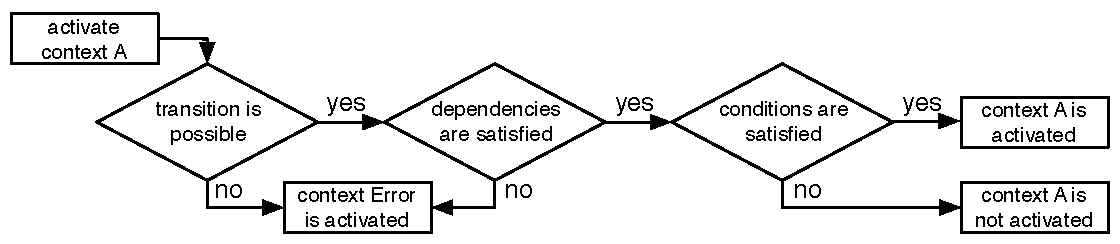
\includegraphics[width=\columnwidth]{pdf/activation_diagram}
}

In general, programmers need to take significant care of context
transitions, in that the latter may drastically change an
application's behavior. To better support programmers in doing so,
every context transition in \conesc entails several checking stages,
as shown in Fig.~\ref{fig:ad}. A successful check allows the
transition to continue, while the failure leads either to the
canceling of the transition or to activation of the \emph{Error}
context. Our translator automatically generates this context unless a
programmer-provided one is explicitly declared in a context group by
using the keyword \code{is error}, as shown on line~\lstref{iserror}
in Fig.~\ref{fig:ccc}.

\putsnippet{
 caption=\emph{NotMoving} context.,
 label=fig:nmc,
 boxname=boxnmc
}

The first check in Fig.~\ref{fig:ad} looks at feasible transitions. In
the context diagram of Fig.~\ref{fig:wtd}, within the \emph{Activity}
group, it is only possible to transition from \emph{NotMoving} to
\emph{Resting}. Feasible transitions are specified within the
individual contexts using the keyword \code{transitions} as in
line~\lstref{transitions} of Fig.~\ref{fig:nmc}. An attempt to
initiate a transition from a given context to one that is not
explicitly listed in the former leads to the activation of the
\emph{Error} context. Indeed, such occurrences typically represent a
significant design or implementation flaw requiring special handling
at run-time, which programmers implement within the \emph{Error} context.

There may also exist relations across context groups. For example,
within the \emph{Base-station} group, a transition from
\emph{Unreachable} to \emph{Reachable} is likely only meaningful if
context \emph{Running} within the \emph{Activity} group is active,
indicating the animal was actually moving when the node gained
base-station connectivity. These inter-group relations are covered in
our design by context dependencies, declared as shown on
line~\lstref{dependence} in Fig.~\ref{fig:cc}. Within the
\code{transitions} clause, the keyword \code{iff} is optionally
employed to indicate the full name of another context whose activation
is required to perform the given transition. The second check in
Fig.~\ref{fig:ad} verifies this rule, again leading to the
\emph{Error} context in case of violations to give programmers an
explicit chance to handle the situation.

The last check in Fig.~\ref{fig:ad} considers violations to ``soft''
requirements that do not necessarily indicate a design or
implementation flaw. Rather, such requirements may be simply needed
for efficiently executing the functionality in a context. For example,
before activating the \emph{Reachable} context, programmers may want
to check that sufficient energy is available to invest in bulk data
transfers to the base-station. Should this not be the case, they may
defer the activation of the \emph{Reachable} context until the solar
panels gather sufficient energy. To implement such processing, \conesc
programmers specify the proper conditions in the body of a predefined
\code{check} command, as shown in line~\lstref{check} of
Fig.~\ref{fig:irc}. If \code{check} returns false, the initiated
context transition does not occur, and the system remains in the
previous context.

\putsnippet{
 caption=\emph{Low} context.,
 label=fig:lc,
 boxname=boxlc
}

Dually, programmers may need to proactively initiate context
transitions as the result of other contexts being activated. The
scenario is symmetric to the previous one: if the base-station is
\emph{Reachable}, but a context transition is initiated to context
\emph{Low} in the \emph{Battery} group of Fig.~\ref{fig:wtd}, the
available energy is running low and it is probably better to refrain
from radio communications even though the base-station is within the
communication range. This makes sure the node does not completely turn
off before the solar panels re-gain energy. Our design allows
programmers to express this processing by using the \code{triggers}
keyword, as shown on line~\lstref{triggers} in Fig.~\ref{fig:lc}. The
\code{triggers} keyword references a context that is to be activated
as the result of the enclosing context being activated. The same
checks shown in Fig.~\ref{fig:ad} apply to this type of transitions as
well.


% Other types of inter-group relations imply automatic triggering of
% context transition. Considering \emph{Battery} group in our example,
% we can notice that for further energy saving developers may want to
% trigger a transition to \emph{Unreachable} context within the
% \emph{Base Station} group as long as \emph{Low} context is active.



%%% Local Variables: 
%%% mode: latex
%%% TeX-master: "bare_conf"
%%% End: 

\section{Evaluation}\label{sec:eval}

We implement three representative applications, as described in
Section~\ref{sec:scenarios}, using either \conesc or nesC. The
implementations are functionally equivalent. Based on these, we
evaluate our approach along three key
dimensions. Section~\ref{sec:evalcomp} analyzes the severity of
different \emph{coupling types} in our implementations. Tighter forms
of coupling, possibly found in multiple instances, are generally
detrimental to code maintenance and
evolution~\cite{stevens79}. Section~\ref{sec:complexity} reports code
metrics assessing the \emph{complexity} of the resulting
implementations, which often impacts a system's reliability and ease
of debugging~\cite{pressman01}. Finally, Section~\ref{sec:overhead}
quantifies the performance overhead, in terms of MCU and memory
penalty, incurred when using \conesc.\lm{At the beginning of a
  structure evaluation section like this one, it's better to give a
  crisp outline of what's coming next, with pointers to the
  subsections.}

Overall, our evaluation reveals that:\lm{Whenever space allows, it's
  useful to summarize the major outcomes of an evaluation
  section. Let's see if we manage to keep it.}
\begin{enumerate}
\item ...
\end{enumerate}

% In this section we show the evaluation of our approach. To this end, we
% developed several scenarios for WSNs and compare nesC implementations against
% its ConesC-written analogs. In addition to the main motivating example shown
% in Sec.~\ref{sec:appdesign}, we describe two more applications for WSNs.

\subsection{Applications}\label{sec:scenarios}

In addition to the wildlife monitoring application we used as a
running example, we implement a smart-home controller and an adaptive
protocol stack to demonstrate the generality of our design.

The smart-home controller, whose design is shown in
Fig.~\ref{fig:shd}, relies on context information to regulate
temperature and lighting conditions in a room, as well as to deal with
emergency situations. The former functionality are driven by
user-provided preferences that depend on the current context. The
preferences are managed within the \emph{Preferences} group, whose
contexts provide different operating parameters depending on day/night
and working days vs.\ weekend conditions. The context transitions
within the \emph{Light} and \emph{Temperature}\lm{We should change
  Climate to Temperature in the diagram.} groups are driven by
thresholds found in such parameter set, compared against current
temperature and light readings. When transitioning between these
contexts, the node operates actuators to control the HVAC and lighting
systems. The controller exploits image, fire, and smoke sensors to
detect housebreaking and fire situations. It may notify the user about
the incident and possibly relay data to a controller in a different
room, depending on the situation.

% The diagram on  displays the possible application of a
% Smart-Home scenario, where each room is supplied with one node. The latter
% detects a \emph{Light} and \emph{Climate} by using corresponding
% sensors. The node uses actuators to adjusts the luminosity and climate according
% to thresholds given by current \emph{Preferences}. The latter depends on the
% time of the day and the day of the week.

% System scenario has CTP backbone and mobile/static nodes around it

\putfigure{caption=Smart-home controller context diagram.,label=fig:shd}{
 \centering
 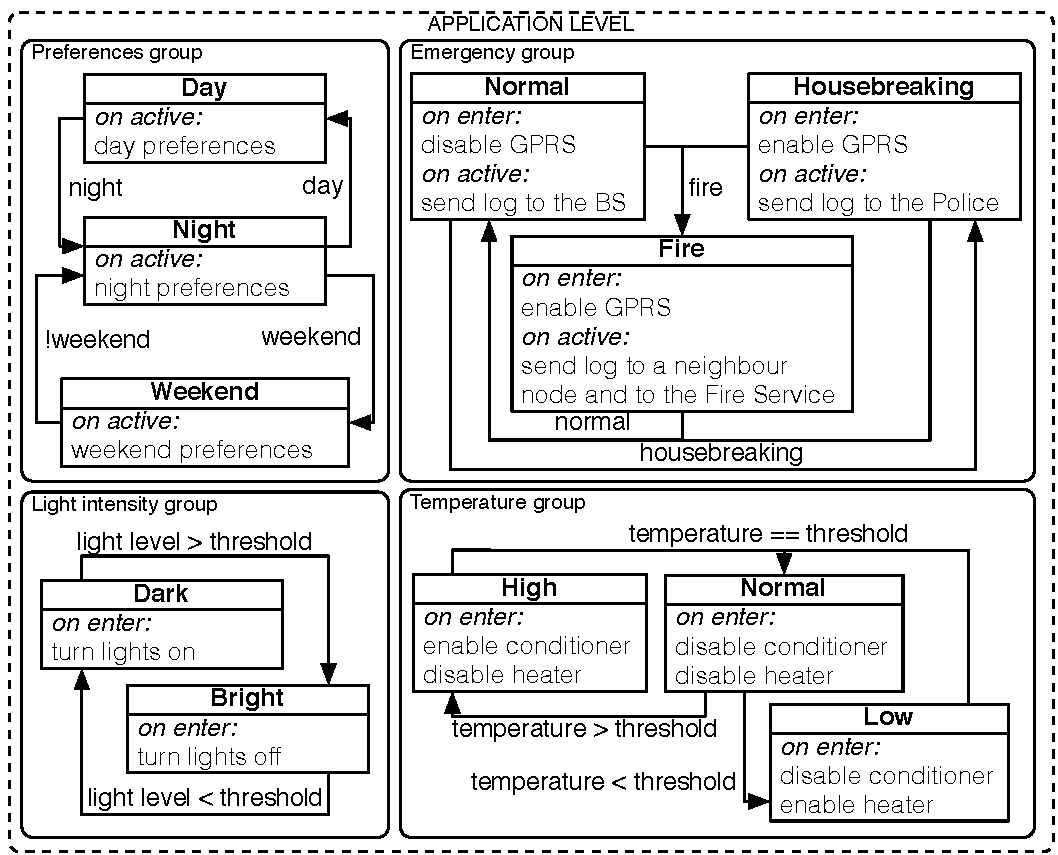
\includegraphics[width=\columnwidth]{pdf/smarthome}
}

The adaptive protocol stack, whose detailed context diagram we omit
for brevity, implements a dynamic protocol switching functionality in
situations where a node may alternative periods of significant
mobility to periods of static operation. The node roams within a
network of static nodes running CTP~\cite{CTP}. As long as the node
remains static, it joins the existing routing tree by running an
instance of CTP limited to being a leaf. As soon as the on-board
accelerometer detects a significant movement, it switches to a simpler
route-less gossip protocol~\cite{gossip}, which allows the node to
relay data to the static infrastructure
opportunistically~\cite{smarthop}. In addition, the node may switch
between three parameter sets for CTP, depending on context information
that determine whether lifetime, bandwidth, or XXXX\lm{Not sure what
  ``link quality adaptation means on the original diagram.} is to be
favored, similar to parameter adaptation in existing MAC protocols
depending on the presence of bursty traffic~\cite{contikiMAC,XMAC}.

% Another scenario - a system-level adaptation - is shown on Fig.~\ref{fig:apd}.
% If the network is static, it is feasible to use a \emph{Collection Tree
% Protocol}. In mobile network, however, a \emph{Gossip}-based protocol shows
% better results. Orthogonally to the \emph{Protocol type}, developer may want to
% adjust the \emph{Protocol parameters} to enhance a link quality between nodes,
% increase the lifetime of the network or use the bandwidth more effectively.

% \putfigure{caption=Adaptive protocol diagram.,label=fig:apd}{
%  \centering
%  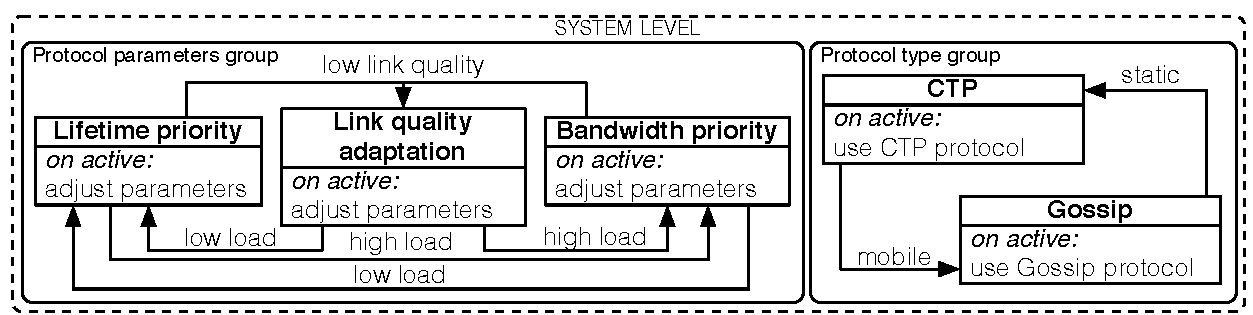
\includegraphics[width=\columnwidth]{pdf/system-level}
% }

\subsection{Coupling}\label{sec:evalcomp}

\begin{table}[!tb]
\renewcommand{\arraystretch}{1.3}
\caption{Coupling types.}
\label{tab:couptypes}
\centering
\begin{tabular}{|l|p{2.5in}|}
\hline
\bfseries Type & \bfseries Description\\
\hline
Content (tightest) & One module relies on the internal working of another. Chang- ing one module requires changes in the other as well.\\
\hline
Common & Two or more modules share some global state, e.g., a variable.\\
\hline
External & Two or more modules share a common data format.\\
\hline
Control & One module controls the flow of another, e.g., passing infor- mation that determine how to execute.\\
\hline
Stamp & Two or more modules share a common data format, but each of them uses a different part with no overlapping.\\
\hline
Data & Two or more modules share data through a typed interface, e.g., a function call.\\
\hline
Message (loosest) & Two or more modules share data through an untyped inter- face, e.g., via message passing.\\
\hline
\end{tabular}
\end{table}

According to Stevens et al.~\cite{stevens79}, seven types of coupling
between software modules exist, as summarized in
Table~\ref{tab:couptypes}. It is generally known that the tightest is
coupling, the more difficult is debugging, maintaining, and extending
the implementations. % Coupling types, which
% are presented in this section, are not forbidden in ConesC, but some
% of them can be easily avoided with a proper use of its concepts.
We investigate the types of coupling in \conesc and the nesC
implementations.

\begin{table}[!tb]
\renewcommand{\arraystretch}{1.3}
\caption{Coupling comparison: \emph{\conesc implementations save most types of coupling that are unavoidable in nesC.}}
\label{tab:coupres}
\centering
\begin{tabular}{|l|l|l|l|l|l|l|l|}
\hline
\bfseries Application & \rotatebox{90}{\bfseries Content} & \rotatebox{90}{\bfseries Common} 
& \rotatebox{90}{\bfseries External} & \rotatebox{90}{\bfseries Control}
& \rotatebox{90}{\bfseries Stamp} & \rotatebox{90}{\bfseries Data}
& \rotatebox{90}{\bfseries Message}\\
\hline
\hline
Wildlife tracking -- nesC &
yes&yes&yes&yes&--&yes&--\\
\hline
Wildlife tracking -- ConesC &
--&--&yes&--&--&yes&--\\
\hline
\hline
Smart-home -- nesC &
yes&yes&yes&yes&--&yes&--\\
\hline
Smart-home -- ConesC &
--&--&yes&--&--&yes&--\\
\hline
\end{tabular}
\end{table}

\fakepar{Results} Table~\ref{tab:coupres}\lm{Can we also count how
  many times we encounter a given type of coupling in either
  implementation?} illustrates the results of our analysis. Generally,
the ConesC implementations are significantly more decoupled compared
to their nesC counterparts.

Specifically, \conesc avoids \emph{Content} coupling in that different
behavioral variations are cleanly encapsulated in different
contexts. NesC programmers, on the other hand, cannot dynamically bind
command calls or event signals to different modules, which forces them
to expose internal module information that make one module's operation
depending on that of several others'. For the same reason, nesC
programmers are forced to use global state to switch between different
functionality depending on the situation. Such global state, which
creates \emph{Common} coupling, is not needed using \conesc, in that
the necessary functionality is automatically generated by our
translator. Finally, \conesc spares \emph{Control} coupling as
well. In essence, this comes as a result of allowing, in a sense,
dynamic binding across modules driven by the context transitions. Such
functionality, which is not available in nesC, needs to be hand-coded
in the latter.\lm{There was no explicit explanation for Common and
  Control... They were not mentioned.}


% Implementation of context components in ConesC, example of which are presented in Fig.~\ref{fig:cc} and~\ref{fig:irc}, do not rely on internal work of each other, so the are not coupled in the sense of~\emph{Content coupling}, as compared to nesC-written application, where all the behavioral variations are encapsulated in one module or function. Since each context represents a separate state of the environment or the device the system operates in, contexts are not intended to share any global states, to control the flow of each other and to pass the information how to execute. Our abstraction toward~\emph{context
% groups} allows developers to perform system-level operations -- e.g. data storage --
% orthogonally to the data processing without actual modules coupling involved.


However, both \conesc and nesC implementations show~\emph{Data}
and~\emph{External} couplings. This is unavoidable, in that different
modules in both implementations must necessarily agree on a common
data format and the C-based nature of nesC favors the use of typed
interfaces to rely on compiler-time type checking.
% We did not use, however, neither messages to share data
% nor different parts of the same data format, so~\emph{Stamp}
% and~\emph{Message} couplings are avoided in both implementations.


\subsection{Complexity}\label{sec:complexity}

We estimate the complexity of the implementations by measuring the
number of variable declarations and the number of functions in every
module. These are generally considered as intuitive indicators of a
program's complexity~\cite{pressman01}. It is also observed that
complexity is a function of the number of states in which the program
can find itself~\cite{35}. A state here is any possible assignment of
values to the program variables. Thus, the number of states must be
computed by looking at the different combinations of values assumed by
variables during every possible execution.

To carry out the latter analysis, we use SATABS~\cite{satabs}, a
model-checking tool for C programs already employed in sensor network
programming for similar analysis~\cite{mottola11survey}. SATABS is
designed for off-line verification of C programs against user-provided
assertions. To do so, it searches through the relevant program
executions to check whether the assertion always holds. At the end of
the process, SATABS returns the number of different states it explores
in the program.  Using a specific configuration, it is possible to
force SATABS to explore \emph{all} program executions. If the
procedure terminates, SATABS returns the total number of distinct
states of the program. We use SATABS on a per-function basis,
implementing empty stubs to replace code that we cannot process with
SATABS, e.g., hardware drivers.

\begin{table}[!tb]
\renewcommand{\arraystretch}{1.3}
\caption{Complexity comparison: \emph{\conesc yields simpler implementations that are easier to debug and to reason about.}}
\label{tab:compres}
\centering
\begin{tabular}{|l|c|c|c|c|c|c|}
\hline
&&&& \multicolumn{3}{@{\hspace{0.3em}}c@{\hspace{0.3em}}|}
{\bfseries Average per-module}\\[0.1in]
\bfseries Application & \rotatebox{90}{\bfseries LOC} 
& \rotatebox{90}{\pbox{0in}{\bfseries Variable\\declarations}} 
& \rotatebox{90}{\bfseries Functions} & \rotatebox{90}{\bfseries LOC}
& \rotatebox{90}{\pbox{0in}{\bfseries Variable\\declarations}}
& \rotatebox{90}{\bfseries Functions}\\
\hline
\hline
Wildlife tracking -- nesC&456&17&19&48&6&8\\
\hline
Wildlife tracking -- ConesC&539(440)&17&30&26,5&3&2\\
\hline
Wildlife tracking -- generated&1628&--&--&--&--&--\\
\hline
\hline
Smart-home -- nesC&360&24&28&28&2&2\\
\hline
Smart-home -- ConesC&382(289)&24&56&13&0,8&1,9\\
\hline
Smart-home -- generated&1310&--&--&--&--&--\\
\hline
\hline
Adaptive protocol -- nesC&150&10&13&38&2,5&3,25\\
\hline
Adaptive protocol -- ConesC&191(147)&5&21&14,7&0,4&1,6\\
\hline
Adaptive protocol -- generated&636&--&--&--&--&--\\
\hline
\end{tabular}
\end{table}

\fakepar{Results} Table~\ref{tab:compres} illustrates our
results\lm{Now that we have good results for the number of states, I
  think we can avoid discussing the implementation-wise numbers and
  LOC.}. On a per-module basis, \conesc shows significant reductions
in both the number of declared variables and defined functions. This
comes from the ability to dynamically bind a function call to the
required context-dependent implementation transparently to the
caller. In nesC, on the other hand, this requires defining global
variables to check what behavior needs to be triggered as a function
of the current situation. As a result of this, the number of
per-function states programmers must manage also decreases
drastically, making the implementations simpler to
understand. Together with the concepts of \emph{contexts}
and~\emph{context groups}, which help in better organizing the code,
this facilitates debugging and maintenance.

%  -- and
% boilerplate code. Because of the same reason, functions have to be
% spitted into smaller isolated parts. We believe, however, that in
% larger applications the number of the similar lines of code will be
% bigger.  

% The number of LOC can also be decreased significantly -- as
% shown in Table~\ref{tab:compres} in parentheses -- by having a tool,
% which generates a boilerplate code using a diagram of a
% context-oriented model of the application, similar to the one
% displayed in Fig.~\ref{fig:wtd}. The logical fragmentation leads to a
% code simplification, improved readability and re-useability along with
% easier debugging and maintaining processes.

As debatable as it may be for measuring the effectiveness of a
programming abstraction~\cite{mottolasurvey}, we also measured the
number of lines of code in both nesC and \conesc implementations. The
two are roughly comparable. More interestingly, we also measured the
size of the code generated by our translator, described in
Section~\ref{sec:translator}, as a measure of the expressive power of
\conesc, that is, the amount of processing that \conesc programmers
can succinctly express using the abstractions we design. It turns out
that the output of our translator is roughly \emph{three times} the
size of the input code, intuitively demonstrating that our
abstractions do capture a significant portion of processing in a few
simple concepts.


% as shown on Table~\ref{tab:compres}, we notice that the
% program written in context-oriented style using plane nesC is more
% than 3 times bigger than its ConesC counterpart. Our approach makes
% context-oriented programming as simple as plain nesC programming.

\subsection{MCU and memory overhead}\label{sec:overhead}

The advantages brought to programmers come at the cost of additional
system overhead. To assess this, we measure the MCU overhead for
context transitions and calls to layered functions, as well as memory
overhead when using \conesc as compared to nesC. To measure the MCU
overhead we use the MSPSim MSP430 emulator~\cite{eriksson09}, while we
estimate the memory overhead using the tools in the nesC and GNU-C
toolchains.

% Since there are neither contexts nor layered functions in nesC-based
% implementation, we measured a number of CPU-cycles of parts with different
% execution flow. For example, contextual events, like a base station presence,
% are detected and handled in ConesC differently as compared to nesC, but,
% eventually, it results in the same functionality. 

\fakepar{Results} Fig.~\ref{fig:cmo}\lm{We should change ``protocol''
  to''stack'' in the picture.} shows the results. The average MCU
overhead for a layered function call ranges from 2 to 5 MCU cycles,
depending on the application. Such figures are negligible in terms of
energy consumption, since the simplest operation in TinyOS, that is
turning on/off an LED, already consumes 8 MCU cycles. The overhead of
context transitions is slightly larger, but in the same order of
magnitude. Most importantly, the memory overhead is also negligible,
measuring a worst-case 2.5\% penalty for the size of the program
binary and a worst-case 4.5\% penalty for RAM usage.\lm{Do we have an
  explanation as to why the adaptive protocol case is the smallest?}

\putfigure{caption=MCU and memory overhead: \emph{the resource usage penalty for using \conesc is almost negligible.},label=fig:cmo}{
\centering
\subfloat[MCU overhead.]{
  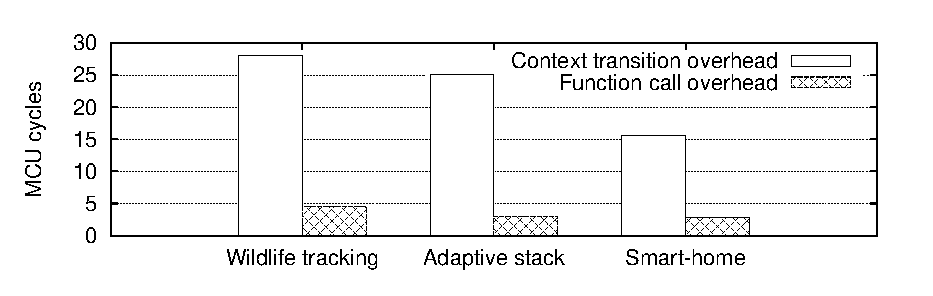
\includegraphics[width =0.5\columnwidth]{pdf/cpu_overhead}
  \label{fig:cpuo}
}
\subfloat[Memory overhead.]{
  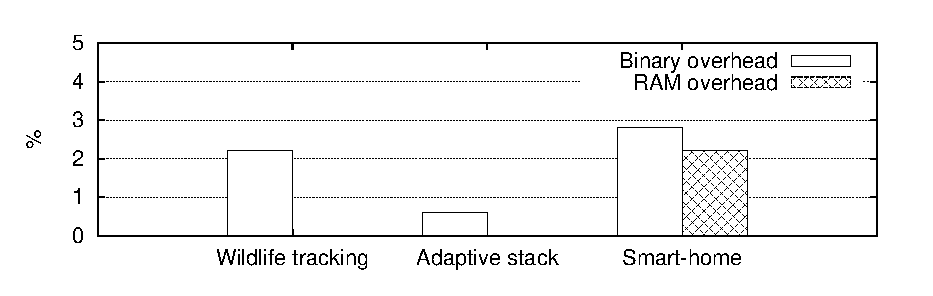
\includegraphics[width=0.5\columnwidth]{pdf/memory_overhead}
  \label{fig:memo}
}
}


%%% Local Variables: 
%%% mode: latex
%%% TeX-master: "bare_conf"
%%% End: 

\section{Conclusion}\label{sec:ending}

We presented programming abstractions for implementing adaptive WSN software. By
borrowing COP concepts, we brought the adaptive software down to low-level
system programming, and introduced a set of language independent concepts,
described in Sec.~\ref{sec:appdesign}. These concepts found their place in our
own context-oriented extension of nesC, called \conesc. To transform \conesc to
plan nesC code, we developed a dedicated translator, described in
Sec.~\ref{sec:translator}.

As we observed in~\ref{sec:eval} based on three representative applications,
\conesc simplifies the developing for WSNs. We shown that along with decoupling
of software components, we gain also a $\approx$50\% reduction in the number of
per-function states that programmers need to deal with. Moreover, due to
decoupled modular structure, \conesc applications can be evolved with lesser
efforts as compared to their nesC counterparts. The price is, however,
negligible: we observed the overhead in memory (data) of maximum 2.5\% (4.5\%),
while the maximum of MCU overhead for context transition (function call) is only
28 (4) MCU cycles.

To our knowledge, efforts related to ours can be divided into WSN-specific
adaptation and programmer support for adaptation outside WSN. Meanwhile, \conesc
brings the design-time programming support for adaptive low-level WSN software.

% use section* for acknowledgement
%\section*{Acknowledgment}
%The authors would like to thank...
\begin{thebibliography}{1}

\bibitem{Bardram05}
J. E. Bardram. \emph{The java context awareness framework (JCAF) – a service infrastructure and programming framework for Context-Aware applications.}, 
In Pervasive Computing, pages 98–115. 2005.

\bibitem{Costanza11}
Costanza P., Hirschfeld R. \emph{Language Constructs for Context-oriented Programming: An Overview of ContextL},
Dynamic Languages Symposium, San Diego, CA, USA, 2005.

\bibitem{Ghezzi10}
Carlo Ghezzi, Matteo Pradella, Guido Salvaneschi \emph{Programming Language Support to Context-Aware Adaptation—A Case-Study with Erlang}, 2010.

\bibitem{Kamina11}
Kamina T., Aotani T., Masuhara H. \emph{EventCJ: a context-oriented programming language with declarative event-based context transition.},
Proceedings of the 10th International Conference on Aspect-Oriented Software Development, AOSD ’11, ACM, New York, NY, USA, pp. 253–264, 2011

\bibitem{Salvaneschi11}
Salvaneschi G., Ghezzi C., Pradella M.
\emph{Towards language-level support for self-adaptive software},
ACM Transactions on Autonomous and Adaptive Systems, 2011.

\bibitem{Salvaneschi12}
Salvaneschi G., Ghezzi C., Pradella M. 
\emph{Context-oriented  programming:  A  software  engineering  perspective},
The  Journal  of  Systems  and  Software, p.1801–1817, 2012.

\bibitem{Sehic11}
Sehic, S., Li, F., Dustdar, S. \emph{COPAL-ML: A Macro Language for Rapid Development of Context-Aware Applications in Wireless Sensor Networks}, 
SENSEA'11, 2011.

\bibitem{Wood08}
A. Wood, J. Stankovic, G. Virone, L. Selavo, Z. He, Q. Cao, T. Doan, Y. Wu, L. Fang, R. Stoleru 
\emph{Context-Aware Wireless Sensor Networks for Assisted-Living and Residential Monitoring}
Network, IEEE  (Volume:22 ,  Issue: 4 ), pp. 26 - 33, 2008.

\end{thebibliography}


% that's all folks
\end{document}


